% brainstorm:

% * citar fundamento em teorias de contornos e pouco uso em composição
% * exemplos das necessidades de operações na composição (peça do mestrado)
% * desenvolvimento do goiaba (para que serve, exemplo de código e de
% saída)
% * trabalhos futuros

\section{Introduction}
\label{sec:introduction}

Contours can be understood as the shape or format of an object. In
Music, they can be associated to elements like pitch, density, rhythm,
and represent a parameter in function of another, as pitch in function
of time. Contours can be easily recognized from graphic representation
by professionals and laymen alike \cite{marvin88:generalized}. For
instance, Beethoven's Fifth Symphony main motive and its pitch contour
are represented respectively in figures \ref{fig:5a-sinfonia-motivo}
and \ref{fig:c-3120}.

\begin{figure}[h!]
  \centering
  \subfloat[Main motive]{
    \includegraphics[scale=.9]{5a-sinfonia}
    \label{fig:5a-sinfonia-motivo}
  }

  \subfloat[Contour (3 1 2 0)]{
    \includegraphics{c-3120}
    \label{fig:c-3120}
  }
  \caption{Fifth Symphony main motive contour}
  \label{fig:5a-sinfonia}
\end{figure}

Contour is defined as an ordered set of distinct elements numbered
from the lowest to the highest \cite{morris93:directions}. In
contours, absolute values of its elements are ignored, and only the
high-low relationship between these elements is regarded. For
instance, figures \ref{fig:5a-sinfonia-motivo} and \ref{fig:ly-3120}
have the same pitch contour, graphically represented in figure
\ref{fig:c-3120}, and symbolically by (3 1 2 0).

The study of Contour is important because, like motives and pitch
sets, contours can help to give coherence to a musical piece. They
represent structural devices that can be combined through operations
like inversion and retrogradation, and can be approached by analytical
or compositional points of view.

\begin{figure}[h!]
  \centering
  \includegraphics{ly-3120-qualquer}
  \caption{A melody with (3 1 2 0) contour}
  \label{fig:ly-3120}
\end{figure}

Contour theories
\cite{friedmann85:methodology,friedmann87:response,morris87:composition,morris93:directions,marvin.ea87:relating,marvin88:generalized,marvin.ea95:generalization,polansky.ea92:possible,quinn97:fuzzy,clifford95:contour,beard03:contour}
have been developed to organize in a systematic way the knowledge
about contour. These theories were developed primarily as analytic
techniques for non-tonal compositions \cite{beard03:contour}, and
provide arrays, matrices and many operations to help the comparison of
contours, like inversion, translation, comparison matrix, and contour
interval array.

Contour operations demand precise mathematical calculations and
graphical representations easy plotting. So a computer program to
process contour can assist composers and analysts in tasks like
operations calculation---avoiding human error and wasting time---,
automated graphical plotting, and conversion from score to contours
and vice-versa. For these reasons we are developing \goiaba{}, a
contour processor software (see section \ref{sec:goiaba}).

\section{The contour processing program Goiaba}
\label{sec:goiaba}

\goiaba{} is a program written in Common Lisp
\cite{graham94:lisp,team07:sbcl} to process and plot contours
developed by the authors of this paper. It has many contour-related
operations, like inversion, retrogradation, rotation, contour
reduction \cite{adams76:melodic}, contour class, contour adjacency
series, contour adjacency series vector, contour interval, contour
interval array, contour class vector I and II
\cite{friedmann85:methodology}, and comparison matrix
\cite{morris93:directions}. Currently, \goiaba{} accepts and shows
contours in a numeric format, but it can also plot contours in a pdf
file.

\goiaba{} has two representations for contours; simple contours
represents only the values of the contour elements, and contour with
durations is basically a collection of cartesian points. For instance,
the contour in figure \ref{fig:c-3120} would be represented as a
simple contour in \goiaba{} as \code{\#s(3 1 2 0)} and as a contour
with duration as \code{\#d(\#p(0 3)\#p(1 1)\#p(2 2)\#p(3 0))}. The
notation \code{\#s(\ldots)} and \code{\#d(\ldots)} indicate a simple
contour and a contour with duration, respectively. The notation
\code{\#p(x y)} indicates a point with two values. So, from the
example we can see that \goiaba{} really represents a contour with
duration as a collection of points. \#s, \#d, and \#p are user-defined
reader macros that expand into code to instantiate objects of types
simple-contour, contour-with-duration, and point, respectively. For
instance, \code{\#(0 1)} is expanded to \code{(make-instance 'point :x
  0 :y 1)}. Finally, \goiaba{} has a few constructor functions besides
the reader macros to help the creation of contour objects. These
functions, \texttt{make-point-list},
\texttt{make-sim\-ple-contour-list}, and
\texttt{make-contour-with-dura\-tion-list}, map a list to the
correspondent object.

\goiaba{} uses the Cl-pdf library\footnote{\url{www.cliki.net/CL-PDF}}
to plot contours, allowing easy visualization of contour operations.
For instance, the following code generates a graph with the original
contour Z, \code{\#s(0 5 3 4 1 3)}, and its retrogradation, inversion,
and rotation. The result can be seen in figure \ref{fig:operacoes}.

\begin{verbatim}
(plot "contour.pdf"
      Z "original Z" :red
      (retrograde Z) "retrograde" :blue
      (inversion Z) "inversion" :orange
      (rotation Z 1) "rotation" :green)
\end{verbatim}

\begin{figure}
  \centering
  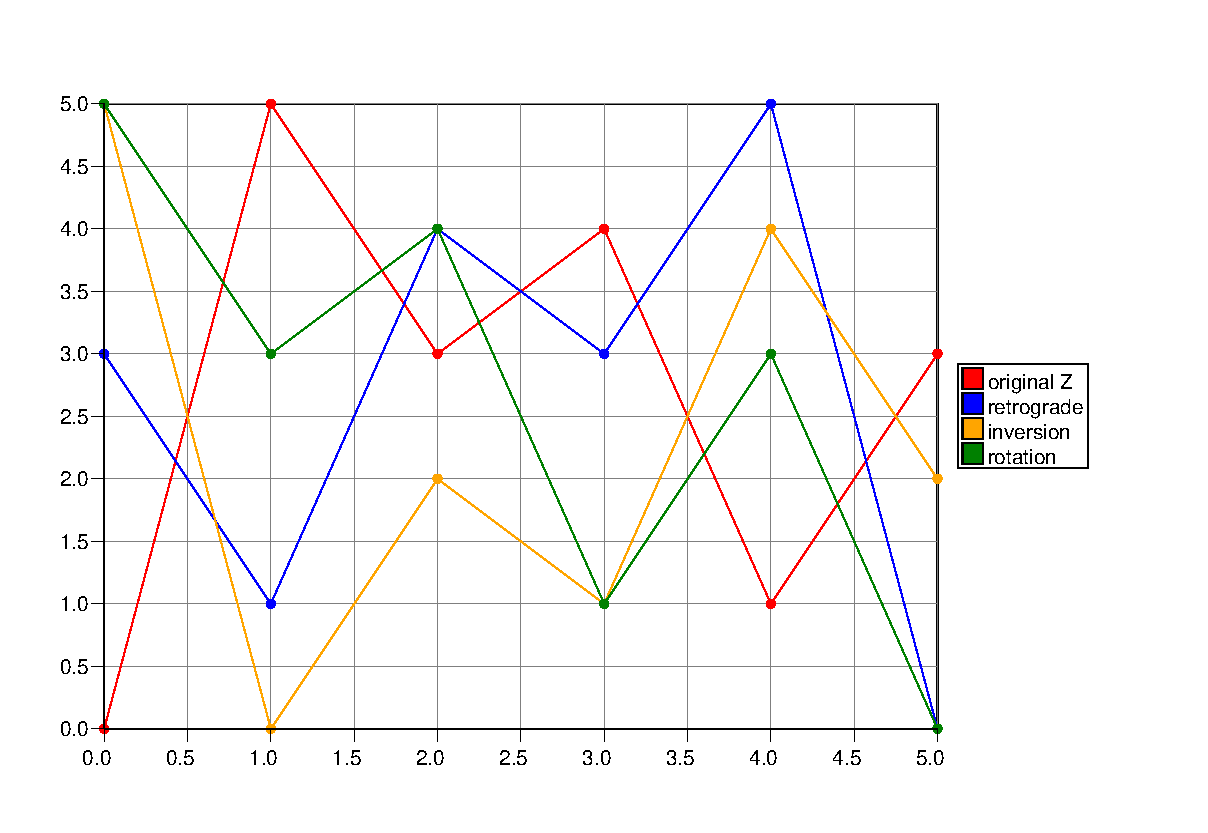
\includegraphics[scale=.44]{contornos}
  \caption{\goiaba{} output: Z(0 5 3 4 1 3) contour operations}
  \label{fig:operacoes}
\end{figure}

\note{write about the advantages of lisp's multimethods}

\note{write small conclusion}

\section{The application of Contour in composition}
\label{sec:cont-appl-comp}

Systematic studies about the usage of contour operations and
combinations in musical composition are scarce, despite the possible
coherence that contours can give and the operations provided by
contour theories. For this reason we are researching contours usage in
composition. The first author of this paper, in his
master's\footnote{The reference was omitted to keep anonymity. It will
  be included in final version.}, composed a woodwind quintet based on
contour theories operations.

This quintet was composed entirely using \goiaba{} to simplify
operations and plotting. The piece is based on combinations of contour
operations associated to parameters such as pitch, tempo, density and
texture. This quintet is based on P(5 3 4 1 2 0) contour
(fig. \ref{fig:c-534120}, its subsets and operations---retrogradation,
inversion, rotation, interpolation.

\begin{figure}
  \centering
  \includegraphics{c-534120}
  \caption{P(5 3 4 1 2 0) contour}
  \label{fig:c-534120}
\end{figure}

\goiaba{} was essential to compose a \eng{fugato}, in the quintet,
because each piece of subject and counter-subject were based on
different combinations of rotation and retrogradation operations.  The
subject has original contour P(5 3 4 1 2 0) and factor 3 rotation
(fig. \ref{fig:sujeito-fugato}). Figure
\ref{fig:output-sujeito-fugato} has the contour software output for
graphical representations of these subject operations. Contour-subject
has original contour retrogradation repeated three times with
different rotation factors---5, 4 and 3
(fig. \ref{fig:contra-sujeito-fugato}). In the same way software
output for these operations are in figure
\ref{fig:output-contra-sujeito-fugato}.

\begin{figure*}
  \centering
  \subfloat[Subject]{
    
\includegraphics[scale=2.8]{sujeito-fugato}
    \label{fig:sujeito-fugato}
  }

  \subfloat[Counter-subject]{
    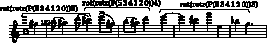
\includegraphics[scale=2.8]{contra-sujeito-fugato}
    \label{fig:contra-sujeito-fugato}
  }
  \caption{Structural elements of \eng{fugato}}
  \label{fig:elementos-fugato}
\end{figure*}

\begin{figure*}
  \centering
  \subfloat[Subject]{
    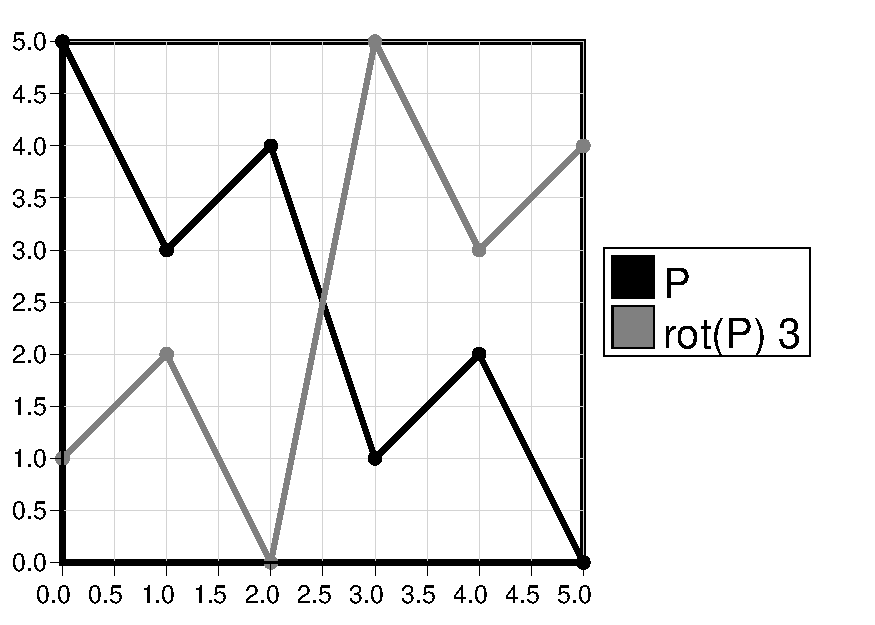
\includegraphics[scale=.44]{output-subject}
    \label{fig:output-sujeito-fugato}
  }
  \subfloat[Counter-subject]{
    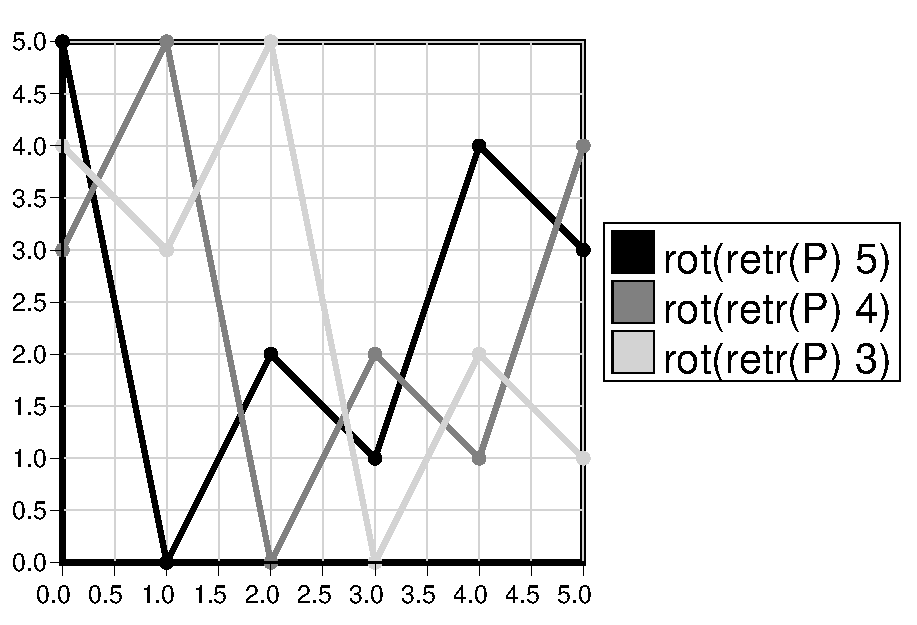
\includegraphics[scale=.44]{output-countersubject}
    \label{fig:output-contra-sujeito-fugato}
  }
  \caption{Software output for \eng{fugato} contour operations}
  \label{fig:output-fugato}
\end{figure*}

\section{Future work}
\label{sec:future-work}

In the future \goiaba{} will receive as input scores in the
Lilypond\footnote{\url{http://lilypond.org/}} format. Lilypond has
conversors from formats as MIDI,
ABC\footnote{\url{http://abcnotation.org.uk/}},
MusicXML\footnote{\url{http://www.musicxml.org/}}, and ETF
Finale\footnote{\url{http://www.music-notation.info/en/formats/ETF.html}}
to its one. As well \goiaba{} will have a graphical interface. The
next step in our research is to improve \goiaba{} user interaction,
releasing a more friendly interface.

%%% Local Variables: 
%%% mode: latex
%%% TeX-master: "goiaba-contour-processor"
%%% End: 